\documentclass[class=scrbook, crop=false]{standalone}
\usepackage[subpreambles=true]{standalone}
\ifstandalone
    % WARNING: Proceed with caution!

% -----------------------------------------------------------------------------------
% For package standalone
% -----------------------------------------------------------------------------------
\usepackage{import}

% -----------------------------------------------------------------------------------
% Language and typeset
% -----------------------------------------------------------------------------------
\usepackage[ngerman, english]{babel}

\usepackage{subcaption}
% Umlauts and other special characters (UTF-8)
% \usepackage[utf8]{inputenc}
\usepackage{fontspec}
\setsansfont{Arial}
% \usepackage[T1]{fontenc}  % Enable accented characters and umlauts
% LuaLatex doesn't need fontenc and uses UTF-8
% \usepackage{lmodern}  % Font face


% --------------------------------------------------------------------------------
% Page formatting
% --------------------------------------------------------------------------------
% Change the header/footer for chapter beginnings and normal pages
\usepackage[automark,headsepline]{scrlayer-scrpage}

% The package provides an easy and flexible user interface to customize the page
% layout, implementing auto-centering and auto-balancing mechanisms
% WARNING: WHEN CHANGING BCOR (Binding correction), the cover needs reworking!...
\newcommand{\theBCOR}{15mm}  % Define binding correction
\usepackage[
    bindingoffset=\theBCOR,
    % showframe, % Show boxes which indicate margins and paddings
    bottom = 3.5cm, % Margins
      left = 2.5cm,
     right = 2.5cm
] {geometry}

% The package 'float' provides a container for document objects which can not be
% broken over pages, such as tables and figures
% Needed for table and figure indexes  
\usepackage{float}

% support for landscape layout
\usepackage{lscape}

% support of \tablenotes command to add notes under table
\usepackage{threeparttable}

% To allow drawing more professional tables
\usepackage{booktabs}

% --------------------------------------------------------------------------------
% Contents
% --------------------------------------------------------------------------------
% Vector graphics (for Cover page)
\usepackage{tikz} 

% Allows additional parameters when including images
\usepackage{graphicx}

% Roman font family for all headings
\addtokomafont{disposition}{\rmfamily}

% Set the line spacing to 1.5
\usepackage[onehalfspacing]{setspace}

% Improves overall text spacing
% http://www.khirevich.com/latex/microtype/
\usepackage[stretch=10]{microtype}

% Math symbols like mu outside the math environment
\usepackage{textcomp}

% A comprehensive (SI) units package∗
% For defining SI units
\usepackage[
    range-units=single,         % Formatting ranges with single unit indication: 1 - 2 m
    range-phrase=-,             % Phrase for range: 1 - 2 m vs 1 to 2 m
    separate-uncertainty=true,  % sets +- between value and uncertainty 
    multi-part-units=repeat     % In expressions with multiple values (multi part numbers) 
                                % the unit is printed each time: 1 mm x 1 mm
] {siunitx}
% https://tex.stackexchange.com/questions/124488/multi-part-numbers-and-units-in-siunitx

% Allows Sourcecodes with highlighting 
\usepackage{listings}

% This package provides user control over the layout of the three basic list
% environments: enumerate, itemize and description
\usepackage{enumitem}
\setlist{nosep} % Remove the vertical space between \item elements in all lists

% ToDo Notes
% \setlength{\marginparwidth}{2cm}
\usepackage{todonotes}
\setuptodonotes{inline, inlinepar}
\reversemarginpar  % Put ToDo notes on the binding's side
% \usepackage{soul} % Colorful ToDo notes

% Check out colors here http://latexcolor.com/
\usepackage{xcolor}

\usepackage{amsmath}    % alignment of equations

% --------------------------------------------------------------------------------
% Other elements
% --------------------------------------------------------------------------------
% Blindtext: Organic looking text dummy
\usepackage{blindtext}

% Hyperlinks within the document (PDF)
% "hidelinks" hides visual highlighting of links
\usepackage[hidelinks]{hyperref}

% Package for Glossary and Index (Acronyms are listed in a separate list) 
\usepackage[acronym, nogroupskip]{glossaries}[=v4.49] % groupskip: alphabetic grouping of entries

\usepackage{xltabular}   % <------- FOR glossaries

% Integration and management of bibliographies
\usepackage{csquotes}   % backend=biber in biblatex needs this package
\usepackage[
    style=ieee,   % style of the bibliography, entries are sorted in alphabetic order. "ieee" is another common style.
    backend=biber,      % based on package 'biber' 
    bibencoding=ascii   % ASCII Text encoding; may use "utf8" instead
] {biblatex}

% --------------------------------------------------------------------------------
%                               PATHS & FILES
% --------------------------------------------------------------------------------
% Fix paths for standalone compiling
\ifstandalone
    \def \home {..}
\else
    \def \home {.}
\fi

% Package: scrlayer-scrpage
% \def \stylePath {\home/settings+/style/page}
\input{\home/settings+/style/page}  % Load page style

% Package: graphicx
\graphicspath{{\home/images/}}  % Set path to images

% Package: listings
\input{\home/settings+/style/code.tex}  % Set path to style file
\lstset{inputpath={\home/code/}} % Default path to code listings

% Package: glossaries
\input{\home/settings+/style/symbols}  % Set path to symbols list style file
\input{\home/settings+/style/acronyms}  % Set path to acronym list style file
% -------------------------------------------------------------------------------
%               Listing of all Glossary and Acronym Entries 
%                           use as shown below
% -------------------------------------------------------------------------------

% ==== EXEMPLARY ENTRY FOR SYMBOLS LIST =========================================

% ==== EXEMPLARY ENTRY FOR ACRONYMS LIST ========================================
% \newacronym{#label}{#acronym}{#long_form}

% define new command for custom arconym entry with only two arguments
% fabricates an easier way to use \newacronym 
\newcommand{\acroX}[2]{\newacronym{#1}{#1}{#2}}
% \acroX{label and arconym}{long name}
% \acroX{CD}               {Compact Disk}

\newcommand{\acroY}[3]{\newacronym{#1}{#2}{#3}}
% \arcoY{label}{acronym}{long name}
% \acroY{CD}   {cd}     {Compact Disk}
 
\newacronym{AEP}{AEP}{Imbalance price}
\newacronym{aFRR}{aFRR}{Automatic Frequency Restoration Reserve}


\newacronym{reBAP}{reBAP}{Uniform imbalance price}
\newacronym{TSO}{TSO}{Transmission System Operator}
\newacronym{FCR}{FCR}{Frequency Containment Reserve}
\newacronym{mFRR}{mFRR}{Manual Frequency Restoration Reserve}
\newacronym{BRP}{BRP}{Balancing Responsible Party}
\newacronym{SB}{SB}{System Balance}
\newacronym{VRE}{VRE}{variable renewable energy}
\newacronym{ID1}{ID1}{intraday index ID1}
\newacronym{MAE}{MAE}{mean average error}
\newacronym{RMSE}{RMSE}{root mean squared error}
\newacronym{MSE}{MSE}{mean squared error}
\newacronym{CRPS}{CRPS}{continuous ranked probabililty score}
\newacronym{GCC}{GCC}{Grid Control Cooperation}
\newacronym{IC}{IC}{Continuous intraday}
\newacronym{VWAP}{VWAP}{volume-weighted average price}
\newacronym{VID}{VID}{traded volume within the intraday market}
\newacronym{ID AEP}{ID AEP}{Intraday Average Energy Price}
\newacronym{FRR}{FRR}{Frequency Restoration Reserve}
\newacronym{TFT}{TFT}{Temporal Fusion Transformer}
\newacronym{DLM}{DLM}{Dynamic Linear Model}
\newacronym{GB}{GB}{Gradient Boosting}
\newacronym{RF}{RF}{Random Forest}
\newacronym{ARIMAX}{ARIMAX}{Autoregressive Integrated Moving Average with eXogenous variables}
\newacronym{xLSTM}{xLSTM}{Extended Long Short-Term Memory}
\newacronym{DWD}{DWD}{Deutscher Wetterdienst}
\newacronym{ENTSO-E}{ENTSO-E}{European Network of Transmission System Operators for Electricity}
\newacronym{IDA1}{IDA1}{Intraday auction 1}
\newacronym{MOSMIX}{MOSMIX}{Model Output Statistics-MIX}
\newacronym{mLSTM}{mLSTM}{memory-optimized LSTM}
\newacronym{sLSTM}{sLSTM}{speed-optimized LSTM}

% ==== EXEMPLARY ENTRY FOR MAIN GLOSSARY ========================================

    % \newglossaryentry{policy}{name={Policy},description={Im geschäftlichen Bereich bezeichnet Policy eine interne Leit- bzw. Richtlinie, die formal durch das Unternehmen dokumentiert und über ihr Management verantwortet wird}}
    % \newglossaryentry{pcie}{name={PCI Express},description={PCI Express („Peripheral Component Interconnect Express“, abgekürzt PCIe oder PCI-E) ist ein Standard zur Verbindung von Peripheriegeräten mit dem Chipsatz eines Hauptprozessors. PCIe ist der Nachfolger von PCI, PCI-X und AGP und bietet im Vergleich zu seinen Vorgängern eine höhere Datenübertragungsrate pro Pin.}}
    % \newglossaryentry{realnumber}
  % Load glossary, symbol and acronyms list

% Package: biblatex
\addbibresource{\home/references/references.bib}  % Set path to bib resources

% Custom variables
\input{\home/settings+/variables}
% --------------------------------------------------------------------------------
%                                   OPTIONAL
% --------------------------------------------------------------------------------


% Simple arithmetic for LaTeX commands
% \usepackage{calc}

% Document Elements
% -------------------

% Index
% \usepackage{imakeidx}

% compact Lists
%\usepackage{paralist}

% visual improvements for citations
% \usepackage{epigraph}

% Create pseudo code
% https://www.overleaf.com/learn/latex/Algorithms
% \usepackage{algorithm}
% \usepackage{algorithmic}
%\usepackage[noend]{algpseudocode}

% Formatting
% -------------------
% Tweaks for scrbook, redefines commands of other packages
% \usepackage{scrhack}

% Intelligent space separator (nice for superscript?)
% \usepackage{xspace}

% Allows breaks within tables
%\usepackage{tabularx}

% Allows for page breaks in tables
% \usepackage{longtable}

% allows modifying of captions
% \usepackage{caption}

% Multiline comments
%\usepackage{verbatim}

% % Custom colors
% \definecolor{dartmouthgreen}{rgb}{0.05, 0.5, 0.06}

% IF you want to define unicode characters
% \DeclareUnicodeCharacter{0229}{\c{e}}
% \DeclareUnicodeCharacter{0306}{\u{Z}}


% Document elements
% ------------------------------------

% Table package
% \usepackage{booktabs}

% Pie diagram
% \usepackage{datapie}

% Side by Side images
% \usepackage{subcaption}

% For landscape tables
%\usepackage{pdflscape}
%\usepackage{afterpage}

% Graphics can be flow around by text
%\usepackage{wrapfig}

\fi
\usepackage[table]{xcolor}% http://ctan.org/pkg/xcolor

% ----------------------------------------------------------------------------
%                               Implementation
% ----------------------------------------------------------------------------
\begin{document}

\chapter{Implementation} % Outline text
\label{Chapter::Implementation}
    This chapter contains a description of how the implemented algorithm works.

% First explain concepts you used in your thesis like filters or methods
% Then explain your approach or algorithm
% Use flowcharts to give an overview
\section{Feature engineering}
\label{Section::Feature_engineering}

The data introduced in section \ref{Chapter::Methodology} can be further refined to gain additional information. 
The following sections contain information about how the data was used to create more features.
Feature engineering was done for energy data, weather data and holiday data.

In the following sections the correlation between features and the imbalance price will be explored.
Using the anderson darling test \ref{andersonAsymptoticTheoryCertain1952} it was confirmed, that the data is normal distributed.
A probability plot for the imbalance price can be seen in figure \ref{fig::rebap_distribution}. 
The red line resembles a normal distribution. 
The imbalance price has a skewness of $27.08$ and a kurtosis of $1194.02$, so the pearson correlation can not be used for analysing correlations.
Instead for the following correlation analyses the spearman rank correlation will be used.

\begin{figure}[ht]
            \centering
            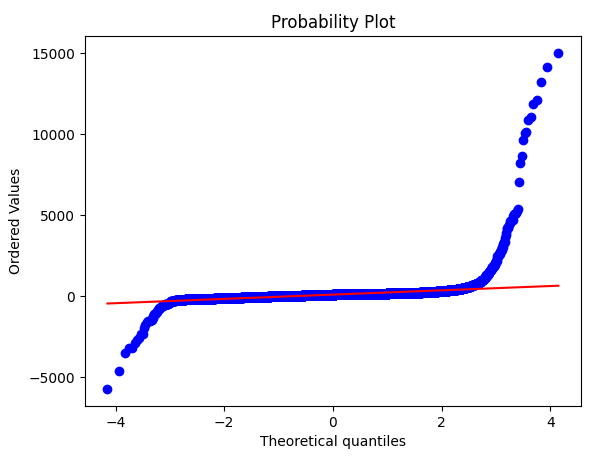
\includegraphics[width=.5\textwidth]{implementation/probability_plot.png}
            \caption[Probability plot for the imbalance price]{Probability plot for the imbalance price}
            \label{fig::rebap_distribution}
 \end{figure}


The imbalance volume and the imbalance price are highly correlated. 
Figure \ref{Figure::volume_price_scatter} shows scatter plots for the imbalance volume and imbalance price.
The correlation coefficient between the imbalance price and the imbalance volume is $0.774$.
In the following subsections the correlation between newly engineered variables and the imbalance price will be inspected.
Due to the high correlation with the imbalance volume, correlations with the imbalance volumes will also be regarded.

\begin{figure}[ht]
            \centering
            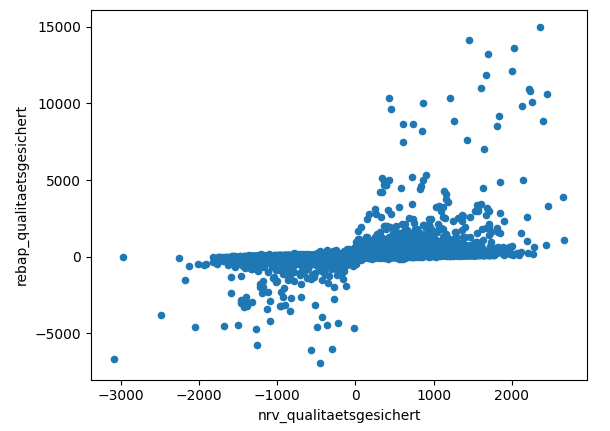
\includegraphics[width=.45\textwidth]{implementation/nrv_rebap_scatter.png}
            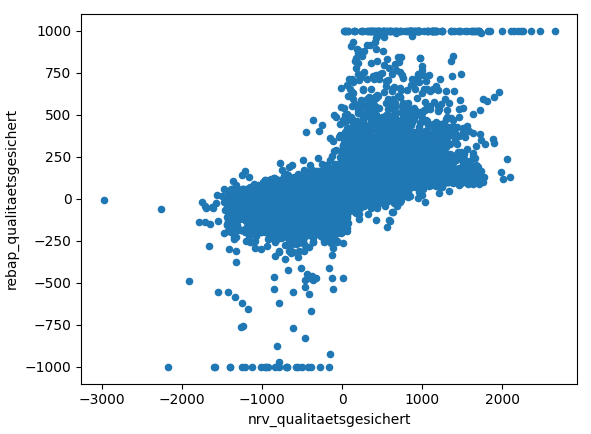
\includegraphics[width=.45\textwidth]{implementation/nrv_rebap_scatter_clipped.png}
            \caption[Scatter plots for imbalance price and imbalance volume. For the plot on the right the imbalane price has been clipped to give information about non-outliers]{Scatter plots for imbalance price and imbalance volume. For the plot on the right the imbalane price has been clipped to give information about non-outliers}
            \label{Figure::volume_price_scatter}
\end{figure}

    \subsection{Energy data}
    \label{Section::FE_Energy_Data}
    The energy data provided by ENTSO-E can be further refined to gain additional information.
    One additional feature is the residual load. 
    Residual load is defined as the load that is not covered by VRE. 
    This is calulated by subtracting the generation provided by solar, wind onshore and win offshore from the load.
    
    Another way of generating more informative features is to calculate the forecasting error. 
    For this the forecast for solar generation, wind generation and load is substracted from the actual measured values.
    This can also be done for the residual load.
    For each of these variables the correlation with the imbalance price is calclulated to estimate how much influence the variables have in determining the imbalance price.
    Table \ref{Table::Rebap_Correlations_ENTSOE} contains the results for these calculations. 
    
    Out of these features the forecasted and actual value for residual load and the residual load forecasting error correlate the most with the imbalance price.
    It should be noted that the actual values apart from the forecasts are not available at prediction time.    

    \begin{table}
    \centering
    \begin{tabular}{l|l|l|l}
    Variable Name	&Forecasted Value& Actual Value	& Forecasting Error \\\hline
    Solar 		& -0.083		& -0.105		& \cellcolor{green} -0.155 \\
    Wind offshore 	& -0.164		& -0.152		& \cellcolor{green} 0.008 \\
    Wind onshore 	& -0.176		& \textbf{-0.189}	& \cellcolor{green} -0.104 \\
    Load 		&0.101		& 0.121		& \cellcolor{green}  0.132 \\
    Residual Load 	& \cellcolor{green} \textbf{0.343}& \cellcolor{green} \textbf{0.391}& \cellcolor{green}0.192\\
    \end{tabular}

    
    \caption{Correlations between variables and \textbf{imbalance price} (rounded to next $10^{-3}$). Green cells are new features}
    \label{Table::Rebap_Correlations_ENTSOE}
    \end{table}

The correlation between the ENTSO-E data and the imbalance volume was calculated as well.
The results for these calculations are displayd in table \ref{Table::Imbalance_volume_Correlations_ENTSOE}. The forecasted and actual value for the residual have a much lower correlation with the imbalance volume than with the imbalance price. The correlation between the residual load forecasting error and imbalance volume is about the same as with the imbalance price. Apart from the load the forecasting error correlates the most with the imbalance volume. 



    \begin{table}
    \centering
    \begin{tabular}{l|l|l|l}
    Variable Name	&Forecasted Value& Actual Value	& Forecasting Error \\\hline
    Solar 		&  -0.011		& -0.024		& \cellcolor{green} \textbf{-0.149} \\
    Wind offshore 	& -0.013		&  -0.022		& \cellcolor{green}\textbf{0.114}\\
    Wind onshore 	& 0.010		& 0.008		& \cellcolor{green} -0.093\\
    Load 		& 0.041		& 0.066		& \cellcolor{green}  -0.040 \\
    Residual Load 	& \cellcolor{green} 0.046& \cellcolor{green} 0.080& \cellcolor{green} \textbf{0.193}\\
    \end{tabular}

    
    \caption{Correlations between variables and \textbf{imbalance volume} (rounded to next $10^{-3}$). Green cells are new features}
    \label{Table::Imbalance_volume_Correlations_ENTSOE}
    \end{table}
    
    The newly introduced features in this section will also be used for inspecting possible features introduced at a later point.
    
    \subsection{Weather data}
    \label{Section::Weather_data}
    The weather data contains a lot of datapoints, especially the MOSMIX forecast. 
    For each of the originally 40 features a forecast is done 240 times for each timestep. 
    This data needs to be condensed, as not all of theses timestamps are useful.
    There are certain timestamps which will be inspected closer for the feature engineering.
    
    The forecasts done by ENTSO-E are published the day before at 18:00. 
    In the MOSMIX data this timestamp will be more closely looked at, because this is the latest forecast available for the forecast made by ENTSO-E.
    Another important timestamp is the latest timestamp. This forecast has access to the most information, thus is most likely the most accurate forecast.
    With a forecast being done each hour, the latest available timestamp at prediction time is the one 2 hours before gate closure time, due to the prediction happening at 1 hour before gate closure time.
    For each of the MOSMIX variables the correlation for both of the previously discussed timestamps is checked.
    
    With both of these configurations for each of the variables a new feature can be created. 
    To get an estimate for the forecasting error in the ENTSO-E data, the change in forecast can be calculated in the DWD data.
    Under the assumption, that a more recent forecast is more accurate, the difference between the latest forecast and the forecast of the day before at $18:00$ is calculated.
    The names for these new features are created by combining a prefix with the abbreviation for the MOSMIX feature.
    For the forecast from the previous day the prefix \textit{DayAhead} is used, the prefix \textit{LastFC} is used for the most recent forecast and \textit{Diff} denotes that the features is the difference between the day ahead forecast and the most recent forecast.
    The results for the correlation analysis between the features and the imbalance can be found in table \ref{Table::imbalance_price_MOSMIX_correlations}. The results for the correlation analysis with the imbalance volume are displayed in table \ref{Table::imbalance_volume_MOSMIX_correlations}.
    The features containing information about wind, namely \textit{FX1} and \textit{FF}, show the highest correlation with the imbalance price. The parameter containing information about cloud coverage (\textit{N05}) is among the highest correlated with both the imbalance price and the imbalance volume. The same is true for the features containing information about solar radiation, \textit{Rad1h} and \textit{SunD1}. In general the correlation between the MOSMIX features and the imbalance volume are a lot lower than the correlations with the imbalance price.
    
    \begin{table}
    \centering
    \begin{tabular}{l|l}
    Variable Name	& Correlation coefficient \\\hline
   	LastFC\_FX1	&-0.254\\
	DayAhead\_FX1	&-0.25\\
	LastFC\_FF		&-0.247\\
	DayAhead\_FF 	&-0.243\\
	DayAhead\_N05	&0.185\\
	LastFC\_N05	&0.176\\
	DayAhead\_wwM	&0.167\\
	LastFC\_wwM	&0.162\\
	LastFC\_Rad1h 	&-0.128\\
	Diff\_Rad1h          	&-0.115\\
	LastFC\_SunD1     	&-0.102\\
    \end{tabular}
    
    \caption{Correlations between feature engineered MOSMIX variables and imbalance price with an absolute correlation coefficient larger than $0.1$ (rounded to next $10^{-3}$)}
    \label{Table::imbalance_price_MOSMIX_correlations}
    \end{table}
    
    \begin{table}
    \centering
    \begin{tabular}{l|l}
    Variable Name	& Correlation coefficient \\\hline
	Diff\_Rad1h                          &-0.08\\
	LastFC\_N05                          &0.074\\
	DayAhead\_N05                        &0.073\\
	Diff\_TTT                           &-0.068\\
	Diff\_SunD1                         &-0.061\\
	Diff\_T5cm                          &-0.055\\
	Diff\_Nl                             &0.052\\
    \end{tabular}
    
    \caption{Correlations between feature engineered MOSMIX variables and imbalance volume (rounded to next $10^{-3}$)}
    \label{Table::imbalance_volume_MOSMIX_correlations}
    \end{table}
    
    
    \begin{table}
    \centering
    \begin{tabular}{l|l}
    Variable Name	& Correlation coefficient \\\hline
	LastFC\_T5cm                        &-0.258\\
	DayAhead\_T5cm                      &-0.253\\
	LastFC\_TTT                         &-0.249\\
	DayAhead\_FF                         &0.246\\
	DayAhead\_TTT                       &-0.243\\
	LastFC\_FF                           &0.233\\
	LastFC\_Nl                           &0.221\\
	DayAhead\_FX1                        &0.216\\
	DayAhead\_Nl                         &0.205\\
	LastFC\_FX1                          &0.204\\
    \end{tabular}
    
    \caption{Correlations between feature engineered MOSMIX variables and residual load forecasting error with an absolute correlation coefficient larger than $0.2$ (rounded to next $10^{-3}$)}
    \label{Table::residual_load_fce_MOSMIX_correlations}
    \end{table}


\section{Data Split}
\label{Section::Data_Split}

To make sure the models trained during the experiments are comparable the models have to be trained and evaulated on the same dataset.
The data was split into a set of training, validation and test data with a share of 70\%, 10\% and 20\% respectively.

For random forest and arima this data split could be done using $train\_test\_split$ from the sklearn package. 
With the more complex Time Series predictors xLSTM and iTransformer needing a different input shape this is a bit more complex.

Instead the training, validation and test split was done along the temporal axis. 
The oldest 70\% were defined as training data, the newest 20\% as test data, with the remaining 10\% being the validation data.


\section{Models}
\label{Section::Models}

In this section implementation details for each of the used models will be discussed. 
The hyperparameter configurations might change during the experiments. 
Any changes done specifically for an experiment will be discussed in the experiment's section.

All the models were implemented in python. 

\subsection{Random Forest}
\label{Section::Random_Forest}

As a random forest regressor the RandomForestRegressor provided by sklearn was used.
Random forest can not use time series data out of the box.
To give some more information about past timesteps shifted features are used.

For the training in the experiments the timesteps of the previous 4 quarter hours were used.

To find the best random forest regressor RandomizedSearchCV by sklearn was used.
In total 20 different parameter combination were tested with a cross validation of 5.
The performance of the models was measured using the negative mean squared error.

\subsection{Arima}
\label{Section::Arima}

For the training of the arima model the module pmdarima was used.
This module provides the function \textit{auto\_arima} to find the best arima model.
The model was trained using the target variable as well as exogenous variables.
The training time increases with the amount of exogenous variables.
For that reason only a subset of features was used for this training.

After the training of a random forest the importance of its features can be extracted using \textit{feature\_importances}. 
The $10$ most important features were used for the training of the arima model.
Using \textit{auto\_arima} the best parameter configuration can be found.

\subsection{xLSTM}
\label{Section::xLSTM}
The configuration for the xLSTM models changes throughout the experiments and will be described in section \ref{Section::Experimental_Setup}

\subsection{iTransformer}
\label{Section::iTransformer}
The configuration for the iTransformer models changes throughout the experiments and will be described in section \ref{Section::Experimental_Setup}



\end{document}
